\documentclass[12pt, centerh1]{article}

\textwidth=165mm \headheight=0mm \headsep=10mm \topmargin=0mm
\textheight=220mm %\footskip=1.5cm
\oddsidemargin=0mm

\RequirePackage[colorlinks,citecolor=blue,urlcolor=blue]{hyperref}
\usepackage{amsmath, amssymb,natbib}

\usepackage{subcaption}
\usepackage{graphicx,bm}
\usepackage{color}
 \usepackage[table]{xcolor}
\usepackage{longtable}
\usepackage{amsthm}
\usepackage[mathscr]{euscript}
\usepackage{relsize}
\newcolumntype{P}[1]{>{\centering\arraybackslash}p{#1}}
\usepackage{rotating}
\usepackage{eurosym}
\usepackage{colonequals}
\usepackage{bbm}
\usepackage{pbox}
\usepackage{booktabs}
\usepackage{dsfont}
\usepackage{authblk}
\usepackage{lscape}
\usepackage{physics}
\usepackage{siunitx}
\usepackage{svg}
\usepackage{float}
\usepackage{multirow}

% Contents of listings-setup.tex
\usepackage{xcolor}
\usepackage{listings}

\lstdefinestyle{mystyle}{
    basicstyle=\ttfamily,
    numbers=left,
    keywordstyle=\color[rgb]{0.13,0.29,0.53}\bfseries,
    stringstyle=\color[rgb]{0.31,0.60,0.02},
    commentstyle=\color[rgb]{0.56,0.35,0.01}\itshape,
    numberstyle=\footnotesize,
    stepnumber=1,
    numbersep=5pt,
    backgroundcolor=\color[RGB]{248,248,248},
    showspaces=false,
    showstringspaces=false,
    showtabs=false,
    tabsize=2,
    captionpos=b,
    breaklines=true,
    breakatwhitespace=true,
    breakautoindent=true,
    escapeinside={\%*}{*},
    linewidth=\textwidth,
    basewidth=0.5em}

\lstset{style=mystyle}

% You can write code using the method below
% Example:
% \lstinputlisting[language=Octave]{BitXorMatrix.m}

% % Uncomment to Exclude All Figures
% % Comment to Include All Figures
% \usepackage{comment}
% \excludecomment{figure}
% \let\endfigure\relax

% Set default image directory
\graphicspath{ {../imgs/} }  


\renewcommand*\abstractname{Abstract}

\title{Application of ARIMA Models in Finance} % 
% Old title: The Evolution of the Goodwin Economics Model
\author{\qquad Karlos Ye$^{1}$ \qquad Grant Forsythe$^{2}$ \qquad Leah Klompmaker$^{3}$}

\date{
{\footnotesize $^1$ Department of Economics and Mathematics, McMaster University, ON, Canada\\[-6pt]
               $^2$ Department of Mathematics and Statistics, McMaster University, ON, Canada\\[-6pt]
               $^3$ Department of Actuarial and Financial Mathematics, McMaster University, ON, Canada\\[-6pt]}
}

%%%%%%%%%%%%%%%
\linespread{1.5}
\pdfminorversion=4

\begin{document}

\maketitle
\vspace{-8mm} % Push abstract up by 8mm
\begin{abstract}
% Example abstract:
In every economy there exist many factors impacting long-term equilibria, some of which have been accounted for by various models. 
Here, we examine the differences between the Goodwin and Goodwin-Keen models which seek to explain economic dynamics. To do so, we present long-term equilibria and conduct a brief sensitivity study. The results illustrate that the Goodwin model presents only one realistic equilibrium, that the Goodwin-Keen model's non-trivial solution is an extreme economic scenario, and that the long-term economic equilibria are impacted by the initial state variable conditions. These findings motivate the pursuit of a deeper understanding of economic dynamics, as it paves the way for better predictions of economic events.

\noindent\textbf{Keywords}: AR, MA, ARIMA, TSA.


\end{abstract}
\newpage

\section{Introduction}
% Introduction Paragragh
Time series analysis has many applications across various industries. With the advancement of technology and ease of access to data, there has been increased investment in end-to-end quantitative and machine learning models that are used to exploit inefficiencies in financial markets \citep{coqueret2021machine}. The purpose of this project will be to analyze historic stock market performance in the US market and fit different models in order to predict near future performance\footnote{Stock market index is calculated as the weighted average of a basket of stocks, representing the overall market performance.}. The S\&P 500 is used to represent the market performance in the United States for the purpose of this study. 
% ; will provide a comparative picture of the different markets and aid in informed decision making for model specification, diagnostics, and finally forecasting. 
% Interpreting the indices movements and forecasting the future values will be a challenging component of this research as stock price movements can be quite dynamic. 
% They can be impacted by many factors concurrently such as interest rates, inflation, economic growth, human behaviour, and international events among others. 

% Body Paragraph
Using historical data to predict the future performance of the index is based on the assumption that stock prices are derived from market forces and historical trends \citep{levy1967relative}. Although this theory was challenged by the Efficient Market Hypothesis proposed by \citet{malkiel2003efficient} which states that stock prices follow a random walk and therefore cannot be predicted by past prices, many empirical studies have found that stock prices are predictable.
% In fact, many hedge fund managers and arbitragers make a living by studying market trends and identifying the most profitable investments for a company. 
% models are one of the most popular linear models and will be considered in this study. ARIMA

% Closing Paragraph
For time series forecasting, there are various techniques that can be applied. In this study, an ARIMA model along with various transformations will be considered to adjust the time series such that it is approximately stationary. This report will conclude by forecasting values of the index based on the model we have fit to the data and remarks are made based on the value of this model as a potential, real-world, predictive tool.

\section{Methodology}
%Karlos Ye
% This is where you write your mathematical definitions, or dataset acquisitions, and or cleaning of data. 

% Specifically, Pandas.DataReader package was used to import data from Yahoo Finance. For example, S&P500 is derived from the weighted average of the stock prices of top 500 U.S firms, with Apple being the most-weighted firm.

\texttt{R} \citep{R} was used to aggregate market data and fit the models.  In this research, the Adjusted Open Price\footnote{Adjusted Open Price is calculated after dividends, stock splits and other factors.} is used as a representation of stock indices data\footnote{The nomenclature follows \citet{cryer2008time}. The entire project can be viewed on \href{https://github.com/grantwforsythe/ARIMA-Model}{GitHub}.}.



\subsection{MA Model}
A moving average process is a finite weighted sum of past random errors plus current random error. A moving average of order $q$, denoted as MA($q$), is defined by
\begin{equation}\label{eq:MA}
    Y_t = e_t - \theta_1e_{t-1} - \theta_2e_{t-2} - \cdots - \beta_pe_{t-q}.
\end{equation}
A strong assumption for MA models is that the time-series is \textit{stationary}, .i.e. the variance and autocorrelation structure do not change with time. 
% where \begin{itemize}
%     \item $\delta$ represents the regression coefficient;
%     \item $e_{t-1},e_{t-2}...e_{t-q}$ represents the past random white noise
% \end{itemize}

\subsection{AR Model}
%An Autoregressive model, as the name suggests, is a regression of itself.% 
In an autoregressive model, the current value from the time series is regressed on the previous value(s) from that same time series. Mathematically, an $p^{\text{th}}$ order autoregressive model, denoted as AR$(p)$, is described by
\begin{equation}\label{eq:AR}
    \centering
    Y_t = \phi_1Y_{t-1} + \phi_2Y_{t-2} + \cdots + \phi_pY_{t-p} + e_t.
\end{equation} 
Like an MA model, AR models require the same assumptions of stationarity.
% where \begin{itemize}
%     \item $Y_t$ represents the current value of the series;
%     \item $\phi$ represents the regression coefficient;
%     \item $Y_{t-1},Y_{t-2}...Y_{t-p}$ represents the past values;
%     \item $e_t$ represents the error term that includes randomness not explained by past values;
% \end{itemize}
% In this model, $\phi_i i \in p \subset \mathbb{Z}$ represents...
% The Goodwin model is described by
% \begin{equation}\label{eq:goodwin} 
% \begin{split}
%     \dot{\lambda} &= \lambda \cdot \left( \frac{1-\omega}{\nu} - \alpha - \beta - \delta \right), \\
%     \dot{\omega} &= \omega \cdot (\Phi(\lambda) - \alpha).
% \end{split}
% \end{equation}
% In this model, $\lambda$ represents the fraction of employed workers, and $\omega$ represents the worker's wage share. The Jacobian matrix for the Goodwin system of equations presented as \eqref{eq:goodwin} is defined by
% \begin{equation} \label{eq:goodwinJ}
% \mathbf J =
% \begin{bmatrix}
%     \pdv{\lambda}\dot{\lambda} & \pdv{\omega}\dot{\lambda}\\[1ex]
%     \pdv{\lambda}\dot{\omega} & \pdv{\omega}\dot{\omega}
% \end{bmatrix}.
% \end{equation}
% This Jacobian matrix was symbolically determined using various methods (i.e. \texttt{solvers.solve}, \texttt{symbols}, \texttt{Matrix}) from the SymPy library \citep{SymPy}.  The equilibrium points and the corresponding eigenvalues of $\mathbf J$ were also symbolically determined using these methods. To corroborate these results, the parameters in Table \ref{tab:parameters} were used to numerically solve the system. This was done using the \texttt{integrate.odeint} method from the SciPy library \citep{2020SciPy-NMeth}. Initial conditions to the system were selected based on \citet{grasselli2012analysis}. The Matplotlib \citep{matplotlib} graphic library was used to generate representative plots of the resulting numerical solution.

\subsection{ARIMA Model}

An Autoregressive Integrated Moving Average, abbreviated as ARIMA, model is a combination of \eqref{eq:MA}, \eqref{eq:AR}, and the number differences required to make the series approximately stationary. Differencing can help stabilize the mean and reduce trends such that the series has relatively constant variance. It takes the linear function of past observations and random error terms to obtain the predicted future value of a predictor.The model is defined as
\begin{equation}\label{eq:ARIMA}
        W_t = \phi_1W_{t-1} + \phi_2W_{t-2} + \cdots + \beta_pW_{t-p} + e_t - \theta_1e_{t-1} - \theta_2e_{t-2} - \cdots - \theta_qe_{t-q}. 
\end{equation}
% We consider the Goodwin-Keen model as the system of differential equations defined by 
% \begin{equation} \label{eq:keen}
% \begin{split}
%     \dot{\lambda} &= \lambda \cdot \left( \frac{\kappa(\pi)}{\nu} - \alpha - \beta - \delta \right),\\
%     \dot{\omega} &= \omega \cdot (\Phi(\lambda) - \alpha),\\
%     \dot{d} &= d\cdot\left(r-\frac{\kappa(\pi)}{\nu}+\delta\right)+\kappa(\pi)-(1-\omega), \\
%     \pi &= 1-\omega-rd.
% \end{split}
% \end{equation}
% Where the newly introduced variable $d$ represents the debt ratio of the economy. Additionally, a nonlinear increasing function $\kappa(\pi)$ now represents a non-linear rate of new investment in the economy \citep{grasselli2012analysis}, and $\pi$ represents the net profits share\footnote{Note, $\pi$ is an implicit part of the model and does not represent a state variable. It represents the net profit made from capital investments \citep{grasselli2012analysis}, and also serves to simplify the analysis.}. The Jacobian matrix for the system is now defined by 
% \begin{equation} \label{eq:keenJ}
% \mathbf J =
% \begin{bmatrix}
%     \pdv{\lambda}\dot{\lambda} & \pdv{\omega}\dot{\lambda} & \pdv{d}\dot{\lambda}\\[1ex]
%     \pdv{\lambda}\dot{\omega} & \pdv{\omega}\dot{\omega} & \pdv{d}\dot{\omega}\\[1ex]
%     \pdv{\lambda}\dot{d} & \pdv{\omega}\dot{d} & \pdv{d}\dot{d}
% \end{bmatrix}.
% \end{equation}
% Given the increased complexity of this model, equilibrium points were determined numerically for a variety of initial conditions using the \texttt{integrate.odeint} method from the SciPy library \citep{2020SciPy-NMeth} and simulating for 1000 steps. The closed-form Jacobian matrix was determined using the SymPy library \citep{SymPy}, and its eigenvalues were then determined using the SymPy \texttt{eigenvects} method. A \emph{basin of attraction} study was then performed on this model using the parameters in Table \ref{tab:parameters}. Long-term model convergence was asserted by verifying that the real part of the eigenvalues of \eqref{eq:keenJ}, for various initial conditions, had a value less than zero. All results were plotted using the Matplotlib \citep{matplotlib} graphic library.

\section{Application}
\begin{itemize}
    \item Show the first difference
    \item Talk about why we aren't using the second difference (over-fitting, more variability)
    \item Fit different ARIMA models
    \item Compare
\end{itemize}
As seen in figure \ref{fig:USA_open} the plot shows a clear upward trend. The variance also tends to be relatively stable with the exception of a few dips.
\begin{figure}[H]
    \centering
    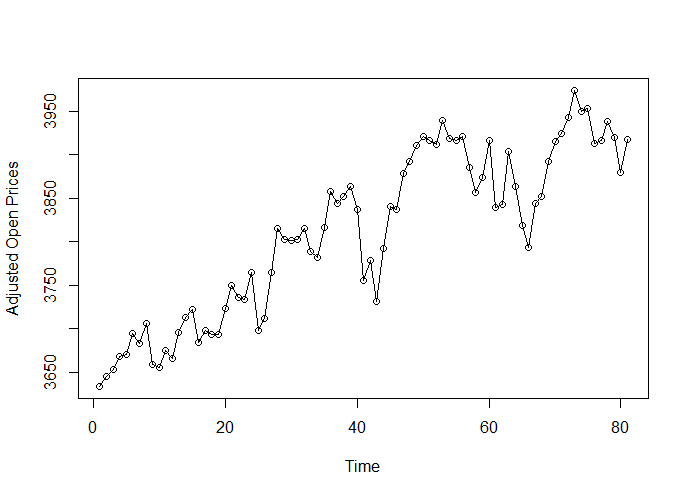
\includegraphics[width=\linewidth]{imgs/USA_open.png}
    \caption{S\&P500 Performance.}
    \label{fig:USA_open}
\end{figure}
As seen in figure \ref{fig:acf}, the autocorrelation function shows that the present value of the series is strongly related to its past values since all lags pictured are significantly out of the confidence band. Interpreting this figure, it indicates that a transformation needs to be performed on the data in order to get to the stationarity assumption.  
\begin{figure}[H]
    \centering
    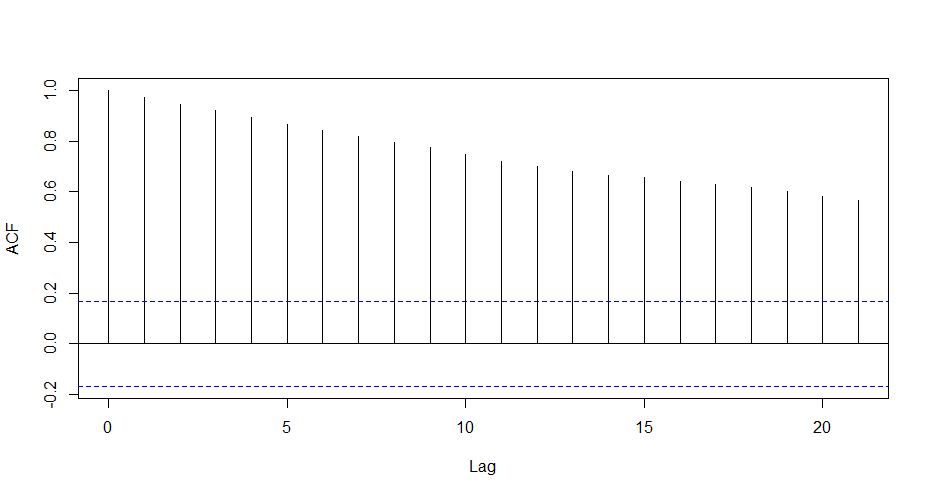
\includegraphics[width=\linewidth]{imgs/acf.png}
    \caption{The ACF of the S\&P500.}
    \label{fig:acf}
\end{figure}
As seen in figure \ref{fig:first_difference}, the first difference is close to having mean zero, and the variance is relatively constant. This suggests that the first difference is a good transformation for this data series as it looks approximately stationary. 
\begin{figure}[H]
    \centering
    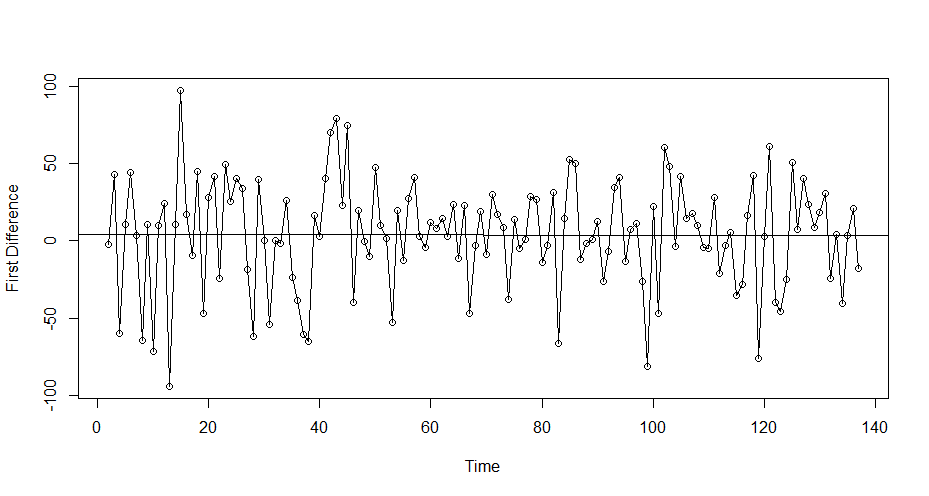
\includegraphics[width=\linewidth]{imgs/first_difference.png}
    \caption{The First Difference of the S\&P500.}
    \label{fig:first_difference}
\end{figure}

\begin{figure}[H]
    \centering
    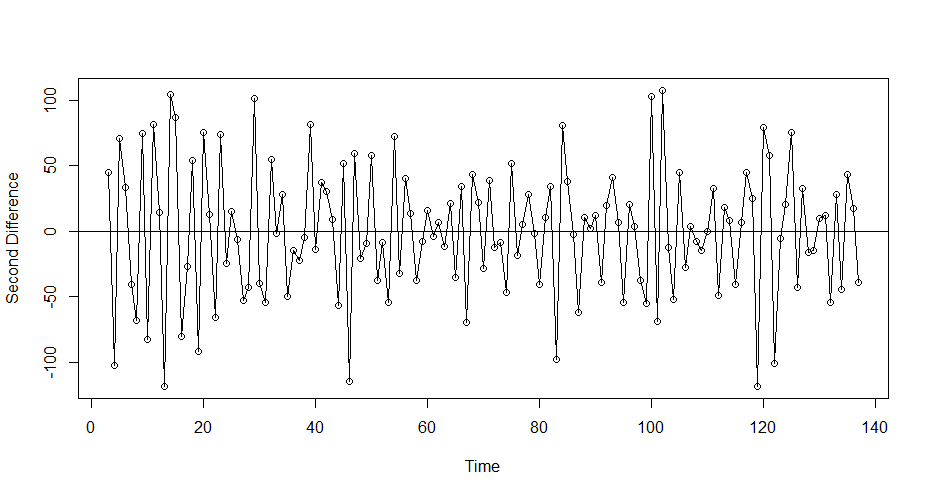
\includegraphics[width=\linewidth]{imgs/second_difference.png}
    \caption{The Second Difference of the S\&P500.}
    \label{fig:second_difference}
\end{figure}

\begin{figure}[H]
    \centering
    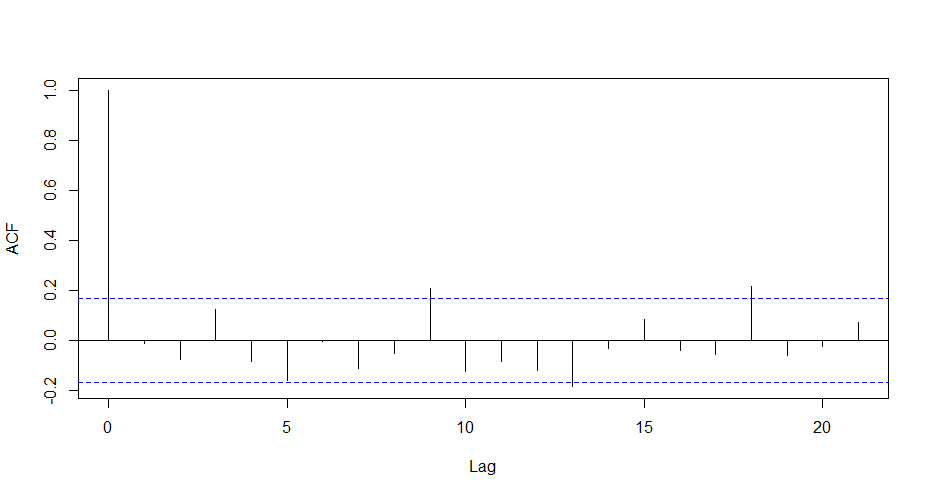
\includegraphics[width=\linewidth]{imgs/acf_first.png}
    \caption{The ACF of the Second Difference of the S\&P500.}
    \label{fig:second_difference}
\end{figure}



% You need to talk about the results of your model. 
% Arthur's Collab. and Synthesized Code: https://colab.research.google.com/drive/1LJISFLnZGBlSe2oGJ1wf6I0rD-wq9Nes?usp=sharing
% The following is a detailed study on the system behaviour demonstrated by the Goodwin model. We begin by noting that in \eqref{eq:goodwin} the Philips curve, $\Phi(\lambda)$, has not been explicitly defined. When the model was proposed \citep{goodwin1982growth}, $\Phi(\lambda)$ was assumed to be a linear function of employment rate. This would mean that a higher fraction of employment leads to a rising wage share. Nevertheless, \citet{goodwin1982growth} admitted that this was an empirical and disputable assumption. On that account, \citet{keen1995finance} proposed \eqref{eq:keenPhil} as a more realistic model. The introduced function models a worker population more willing to accept wage cuts at higher levels of unemployment (i.e. lower $\lambda$). Conversely, as employment rates increase, workers will demand real wages that asymptotically increase (i.e. $\lambda\to1$). This function was also adopted by \citet{grasselli2012analysis} and incorporated into the Goodwin model
% \begin{equation} \label{eq:keenPhil}
%     \Phi(\lambda) = \frac{\Phi_1}{(1-\lambda)^2}-\Phi_0.
% \end{equation}
% Thus, from \eqref{eq:goodwinJ}, it follows that
% \begin{equation} \label{eq:jac_good}
%     \mathbf J = \begin{bmatrix}
%         \frac{1-\omega}{\nu}-\alpha-\beta-\delta & -\frac{\lambda}{\nu}\\[1ex]
%         \frac{2\Phi_1\omega}{(1-\lambda)^3} & \frac{\Phi_1}{(1-\lambda)^2}-\Phi_0-\alpha
% \end{bmatrix}.
% \end{equation}
% The eigenvalues of \eqref{eq:jac_good} determine the nature of the stability of the model at equilibrium. As it turns out, the Goodwin model has two equilibrium points besides the trivial solution $(\lambda^\ast,\omega^\ast)=(0, 0)$. These include
% \begin{equation} \label{eq:goodwin_eqm}
% \begin{split}
%     (\lambda_\pm^\ast, \omega^\ast) &= \left(1\pm\sqrt{\frac{\Phi_1}{\alpha + \Phi_0}},\quad  1-\nu\cdot(\alpha + \beta + \delta)\right)
% \end{split}.
% \end{equation}
% We first must note that all the parameters in \eqref{eq:goodwin_eqm}, as described in Table \ref{tab:parameters}, are positive such that $\sqrt{\frac{\Phi_1}{\alpha + \Phi_0}} \in\mathbb R > 0$. Moreover, $\lambda$ is restricted to the bounded interval $[0, 1]$. This means the only economically feasible equilibrium point is $(\lambda_-^\ast, \omega^\ast)$, since $\lambda_+^\ast$ is inevitably greater than unity. As $(\lambda_-^\ast, \omega^\ast)$ is the only meaningful equilibrium point, we simply denote it as $(\lambda^\ast, \omega^\ast)$. The valid equilibrium point can be incorporated into \eqref{eq:jac_good} and yield the following eigenvalues
% \begin{equation} \label{eq:goodwin_eig}
%     \pm\sqrt 2\cdot\sqrt{\xi_1 - \xi_2},
% \end{equation}
% where
% \begin{equation*}
% \begin{split}
%     \xi_1 &= \frac{\Phi_0 + \alpha}{\nu} + \frac{\sqrt{\Phi_1\cdot(\Phi_0 + \alpha)}(\Phi_0+\alpha)(\alpha+\beta+\delta)}{\Phi_1},\\
%     \xi_2 &= \frac{\sqrt{\Phi_1\cdot(\Phi_0 + \alpha)}(\Phi_0 + \alpha)}{\Phi_1\nu} + (\Phi_0+\alpha)(\alpha+\beta+\delta).
%     \end{split}
% \end{equation*}
% These expressions hold an integral detail about the nature of the equilibrium points. Namely, whether the solution is cyclic in nature. Clearly, if $\xi_1>\xi_2$ then the eigenvalues are solely real and must necessarily diverge (since one of the eigenvalues is strictly positive). However, if $\xi_1<\xi_2$ we can guarantee that both eigenvalues will yield a converging solution, and said solution will be cyclical in nature. Importantly, scenario one, while mathematically plausible, is also economically unrealistic because it suggests that either $\lambda$ or $\omega$ must exceed unity. To proceed, the parameter values defined in Table \ref{tab:parameters} are introduced. Evaluating expression \eqref{eq:goodwin_eig} yields the (approximate) imaginary eigenvalues $\pm0.747558\sqrt{2}i$.
% With these parameters we can also determine the equilibrium point to be approximately
% \begin{equation}
%     (\lambda^\ast, \omega^\ast) = (0.968612, 0.835000).
% \end{equation}
% \noindent
% To verify the aforementioned results, the system was numerically solved. Figure \ref{fig:goodwin} shows the behaviour of the model for 100 steps (equivalent to 100 years). 
% \begin{figure}[H]
%     \centering
%     \includesvg[scale=0.7]{goodwin_model.svg}
%     \caption{Goodwin Model Limit Cycle, Simulated for 100 Steps.}
%     \label{fig:goodwin}
% \end{figure}
% \noindent With the selected parameters, the model must be convergent and exhibit a cyclical behaviour. This behaviour is clearly demonstrated by the phase portrait depicted in Figure \ref{fig:goodwin_phase}. Here, the model was simulated for 1000 steps, and it is evident that the system, while not static, had reached a form of equilibrium; particularly a limit cycle. This plot also shows the value of the equilibrium point $(\lambda^\ast, \omega^\ast)$ relative to the equilibrium orbit of the system.
% \begin{figure}[H]
%     \centering
%     \includesvg[scale=0.7]{goodwin_phase.svg}
%     \caption{Phase Portrait of the Goodwin Model Limit Cycle, Simulated for 1000 Steps.}
%     \label{fig:goodwin_phase}
% \end{figure}

% \subsection{The Goodwin-Keen Model}
% The Jacobian matrix for the Goodwin-Keen model makes use of both \eqref{eq:keenPhil} and 
% \begin{equation*} \label{eq:keenKappa}
%     \kappa=\kappa(\pi) = \kappa_0 + \kappa_1\mathrm e^{\kappa_2\pi}.
% \end{equation*}
% Before we present the matrix, we note the use of the notational simplification
% \begin{equation*}
%     \kappa^\prime = -\pdv{\kappa}{\omega} = -\frac{1}{r}\pdv{\kappa}{d} = \kappa_1\kappa_2\mathrm e^{\kappa_2\pi}.
% \end{equation*}
% Thus the Jacobian matrix for the Goodwin-Keen model is given by
% \begin{equation} \label{eq:jac_keen}
%     \mathbf J = %
%     \begin{bmatrix}
%         \frac{\kappa-\nu(\alpha+\beta+\delta)}{\nu} & -\frac{\lambda\kappa^\prime}{\nu} & -\frac{\lambda r\kappa^\prime}{\nu} \\[0.5em]
%         \frac{2\Phi_1\omega}{(1-\lambda)^3} & \frac{\Phi_1}{(1-\lambda)^2}-\Phi_0-\alpha & 0\\[0.5em]
%         0 & \frac{(d-\nu)\kappa^\prime+\nu}{\nu} & \frac{r\cdot(d-\nu)\kappa^\prime}{\nu}+ \delta + r
%     \end{bmatrix}.
% \end{equation}
% The numerical solution provided values for the equilibrium points. One illustrative example of the solution of the model is shown in Figures \ref{fig:keen} and \ref{fig:keen_phase} using the parameter values in Table \ref{tab:parameters} and initial conditions used by \citet{grasselli2012analysis}.
% \begin{figure}[H]
%     \centering
%     \includesvg[scale=0.7]{keen_model.svg}
%     \caption{Goodwin-Keen Model Convergence to Equilibrium Points, Simulated for 300 Steps.}
%     \label{fig:keen}
% \end{figure}

% \begin{figure}[H]
%     \centering
%     \includesvg[scale=0.7]{keen_phase.svg}
%     \caption{Goodwin-Keen Equilibrium Three-dimensional Phase Diagram.}
%     \label{fig:keen_phase}
% \end{figure}
% \noindent The results of the simulation study for the basin of attraction of this model are consolidated in Figure \ref{fig:keen_study}.
% \begin{figure}[H]
%     \centering
%     \includesvg[scale=0.7]{keen_study.svg}
%     \caption{Goodwin-Keen Basin of Attraction.}
%     \label{fig:keen_study}
% \end{figure}
% \noindent This figure shows that, of the total 1000 simulations performed, only 102 sets of initial conditions converged, and the remaining 898 did not. Moreover, all converging events lead to the same equilibrium point
% \begin{equation}
%     (\lambda^\ast, \omega^\ast, d^\ast) = (0.968612, 0.86053, 0.070191).
% \end{equation}
% The simulations that lead to a diverging event yielded floating-point values where $\lambda$ and $\omega$ were consistently on the order of \num{e-20} (or lower) and $d$ on the order of \num{e19} (or higher). This suggests that another ``equilibrium point'' can be found at
% \begin{equation}
%     (\lambda^\times, \omega^\times, d^\times) = (0, 0, +\infty).
% \end{equation}

\subsection{Model Comparison} 
% It is known that the Goodwin model suffers from many limitations \citep{harvie2000testing, moura2013testing}. Nevertheless, the model has persisted. The Goodwin model supplies economists with insight into the prey-predator relationships between capitalists and workers \citep{goodwin1982growth}. We have concluded from our study that this model only has one economically realistic equilibrium. More importantly, this equilibrium can only be divergent (but economically unfeasible) or oscillatory. This feature has been heavily criticized since, in reality, economies are liable to failures. The Goodwin model does not consider such a scenario, as it does not describe the economy in sufficient detail. However, what it does offer is a concise formulation and a stepping-stone for more complex and accurate models.

% Such is the case for the Goodwin-Keen model. What Steve Keen accomplished was the persistence of the prey-predator nature of the original model with the possibility of exhibiting an economic failure scenario \citep{keen1995finance}. Here, $(\lambda^\times, \omega^\times, d^\times)$ represents this critical contribution to the overall model. Unlike with the Goodwin model, where the trivial solution holds no economic value, the divergent solution for the Goodwin-Keen model describes the real scenario of an economy with maximum debt, absolute unemployment, and no wage share for the working population \citep{minsky1992financial}. Our simulation study also shows that \emph{ceteris paribus}, the nature of the long-term equilibrium of the economy, is dependent on the initial conditions of the state variables $\lambda$, $\omega$, and $d$. That is, economies described by the same parameters can fail or stabilize solely as a result of where they begin.

% If your model or problem set has parameters your change, this is where you would write about it. 
% Minimum 1 and a half pages. 

\section{Conclusion}
Throughout this report, the Goodwin and Goodwin-Keen models have been described qualitatively, and presented mathematically. The behaviours of the economic models have been explored numerically and analytically. The tendency of the Goodwin model to converge to an oscillatory equilibrium state or diverge has been demonstrated. The Goodwin-Keen model, which can show more realistic features representative of an economic collapse, has been investigated, and simulations have been performed. A thorough comparison of the models has interpreted their behaviours. This study has concluded that the Goodwin model produces unrealistic long-term behaviour that cannot be used to accurately describe an economy. It has, however, led to many more economically representative models based on the original prey-predator dynamic, such as the Goodwin-Keen model. As demonstrated in this report, Keen's improved model can reasonably simulate an economic crash (instability). The ability to simulate and predict an incoming economic crash, such as a recession or depression, gives governments invaluable foresight. This may allow policy-makers to enact regulations for avoiding, or at the very least, curbing the severity of the crash. Our findings motivate the pursuit of a deeper understanding of economic dynamics, as it paves the way for better predictions of economic events.
% Housing Prices: Future projections show this, from the model. Then write about what the future results indicate. 
% SIR Model: If you decrease the infection rate by 20\%, you will get a peak decrease of 15\%. 
% Sport Statistics: This model indicates player outcomes for this and this team to win these type of games. 
% This is half a page long.

% \section{Acknowledgments}
% We would like to thank Dr. Cousins (McMaster University) for his guidance throughout the project.

\nocite{*}
\bibliographystyle{chicago}
\bibliography{bibliography.bib}
\newpage

\section{Appendix}
\lstinputlisting[caption={R Commands.}, language=Python]{../scripts/getdata.py}

% \newpage
% \section*{Appendix}

\end{document}
